% \mysection{5}{METODOLOGÍA}
\section{METODOLOGÍA}

Para poder diseñar una arquitectura de microservicios efectiva, correcta y que responda a las
necesidades del negocio se propone una metodología iterativa que se compone de cinco etapas:


\subsection{Identificar el dominio del negocio}

Puede sonar como un axioma sin sentido, después de todo ¿qué negocio no sabe cuál es su dominio?
Sin embargo muchos arquitectos expertos siempre aconsejan empezar por aquí debido a que si bien los
expertos del dominio conocen la parte de negocio en la cual se desenvuelven, es altamente probable
que no conozcan los detalles del cómo funciona el negocio fuera de sus actividades cotidianas.

En concreto, un empleado del departamento de ventas puede conocer muy bien sus responsabilidades
y funciones dentro del flujo de ventas.
Además conoce relativamente bien las responsabilidades y funciones de los departamentos con los que más
interacción tiene (para este ejemplo almacén).
Sin embargo no conoce de los detalles de las funciones que estos otros departamentos cumplen, específicamente
no conoce de la cantidad exacta de productos que existen físicamente en almacén, no conoce los horarios
de reaprovisionamiento, no sabe que desde la semana pasada almacén tiene un nuevo vehículo que hará que
el trabajo sea más rápido.

El escenario mencionado se repite departamento a departamento, unidad de trabajo a unidad de trabajo
a lo largo y ancho de toda la organización.
Es debido a esto que es probable que la organización no tenga en claro específicamente qué acciones
son las que entregan valor y por lo tanto identificar el dominio del negocio debe ser el punto de inicio
para el equipo de desarrollo.

\subsubsection*{Entradas}
\begin{enumerate}[a.]
	\item Documentos internos de la empresa.
\end{enumerate}

\subsubsection*{Técnicas y herramientas}
\begin{enumerate}[a.]
	\item Reuniones multi-departamentales.
	\item Revisión de documentos internos.
	\item Seguimiento de flujo de producto.
\end{enumerate}

\subsubsection*{Salidas}
En esta etapa no existen salidas concretas debido a que lo único que se quiere es que el equipo
de desarrollo entienda en un nivel alto el dominio de la empresa u organización.

\subsection{Diseño Guiado por el Dominio}

En esta etapa utilizaremos las pautas que nos da el diseño basado en dominios.
Se utiliza este marco porque ya fue probado múltiples veces en el mundo real para ir desde
el nivel más alto de la aplicación hasta definir los detalles de organización de los microservicios.

Debido a que se propone una metodología iterativa para refinar los microservicios, el marco de trabajo
de diseño basado en dominios tiene la ventaja de que también está pensado como un proceso iterativo
por lo cual es congruente a la metodología propuesta.

\subsubsection{Análisis del Dominio}

El equipo de desarrollo ya tiene una idea general de qué es el dominio del negocio, pero no tiene
nada formal con lo que empezar a implementar la solución.
Entonces lo que se debe hacer es crear un modelo del dominio.
Este modelo permite ver el dominio del negocio de manera holística para poder identificar
los sub-dominios núcleo, los subdominios de soporte y los subdominios genéricos.

Para identificar correctamente el modelo de dominio de la organización es necesaria la participación
de todos los departamentos.
La gerencia debe apoyar para garantizar la participación de toda la organización en el modelado del dominio.

Se requiere una participación total debido a que si bien cada departamento, oficina o equipo son expertos
en sus dominios aislados y sea tentador el modelar el dominio basándose en las divisiones que la organización ya
tiene, el modelo corre peligro de ser contradictorio y el diccionario de términos estar incompleto.

Si se comete el error de intentar modelar el dominio departamento por departamento, no se encontrarán
conflictos de flujo interdepartamentales, también es altamente probable que en el modelo de dominio
se separen elementos que realmente tienen alta cohesión generando problemas de dependencia en el futuro.
Además de los problemas que genera al modelo, el diccionario de términos que sirve para que el equipo
de desarrollo y los expertos del dominio puedan comunicarse efectivamente, quede incompleto o tenga
términos incorrectos o tenga términos contradictorios entre departamentos o en el peor de los casos
todo lo anterior mencionado.

\subsubsection*{Entradas}
\begin{enumerate}[a.]
	\item Flujo de valor informal de la organización.
\end{enumerate}

\subsubsection*{Técnicas y herramientas}
\begin{enumerate}[a.]
	\item Cuadros de dominios.
  \item Event storming
\end{enumerate}

\subsubsection*{Ejemplo de la técnica cuadro de dominio}
\vspace{1em}

  \begin{figure}[H]
    % \caption{\\\hspace{\textwidth} Ejemplo de un cuadro de dominio}
    \caption{Ejemplo de un cuadro de dominio}
    \centering
    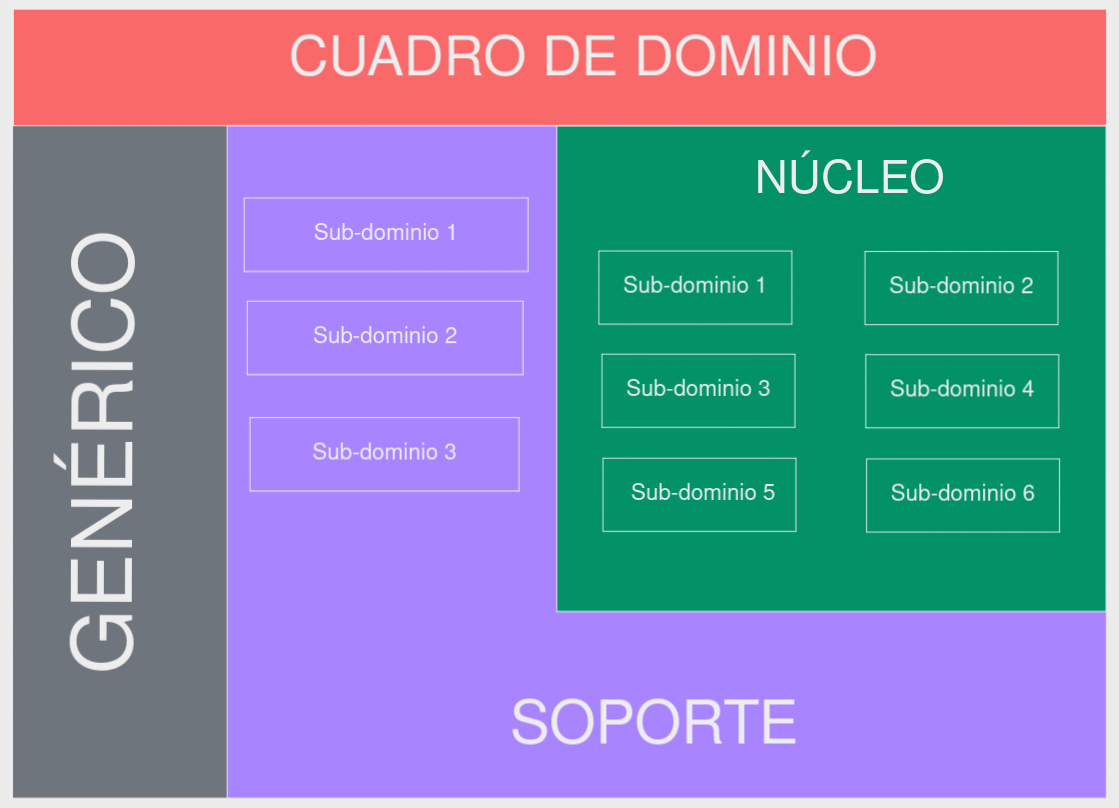
\includegraphics[width=0.90\textwidth]{src/assets/metodologia/cuadro_dominio}
    \label{fig:cuadro_dominio}
    \\
    Nota: Gráfica de ejemplo de un cuadro de dominio. Elaboración propia.
  \end{figure}


\subsubsection*{Ejemplo de la técnica event storming}
\vspace{1em}

  \begin{figure}[H]
    % \caption{\\\hspace{\textwidth} Ejemplo de un cuadro de dominio}
    \caption{Ejemplo de un cuadro producto de una reunión de event storming}
    \begin{center}
    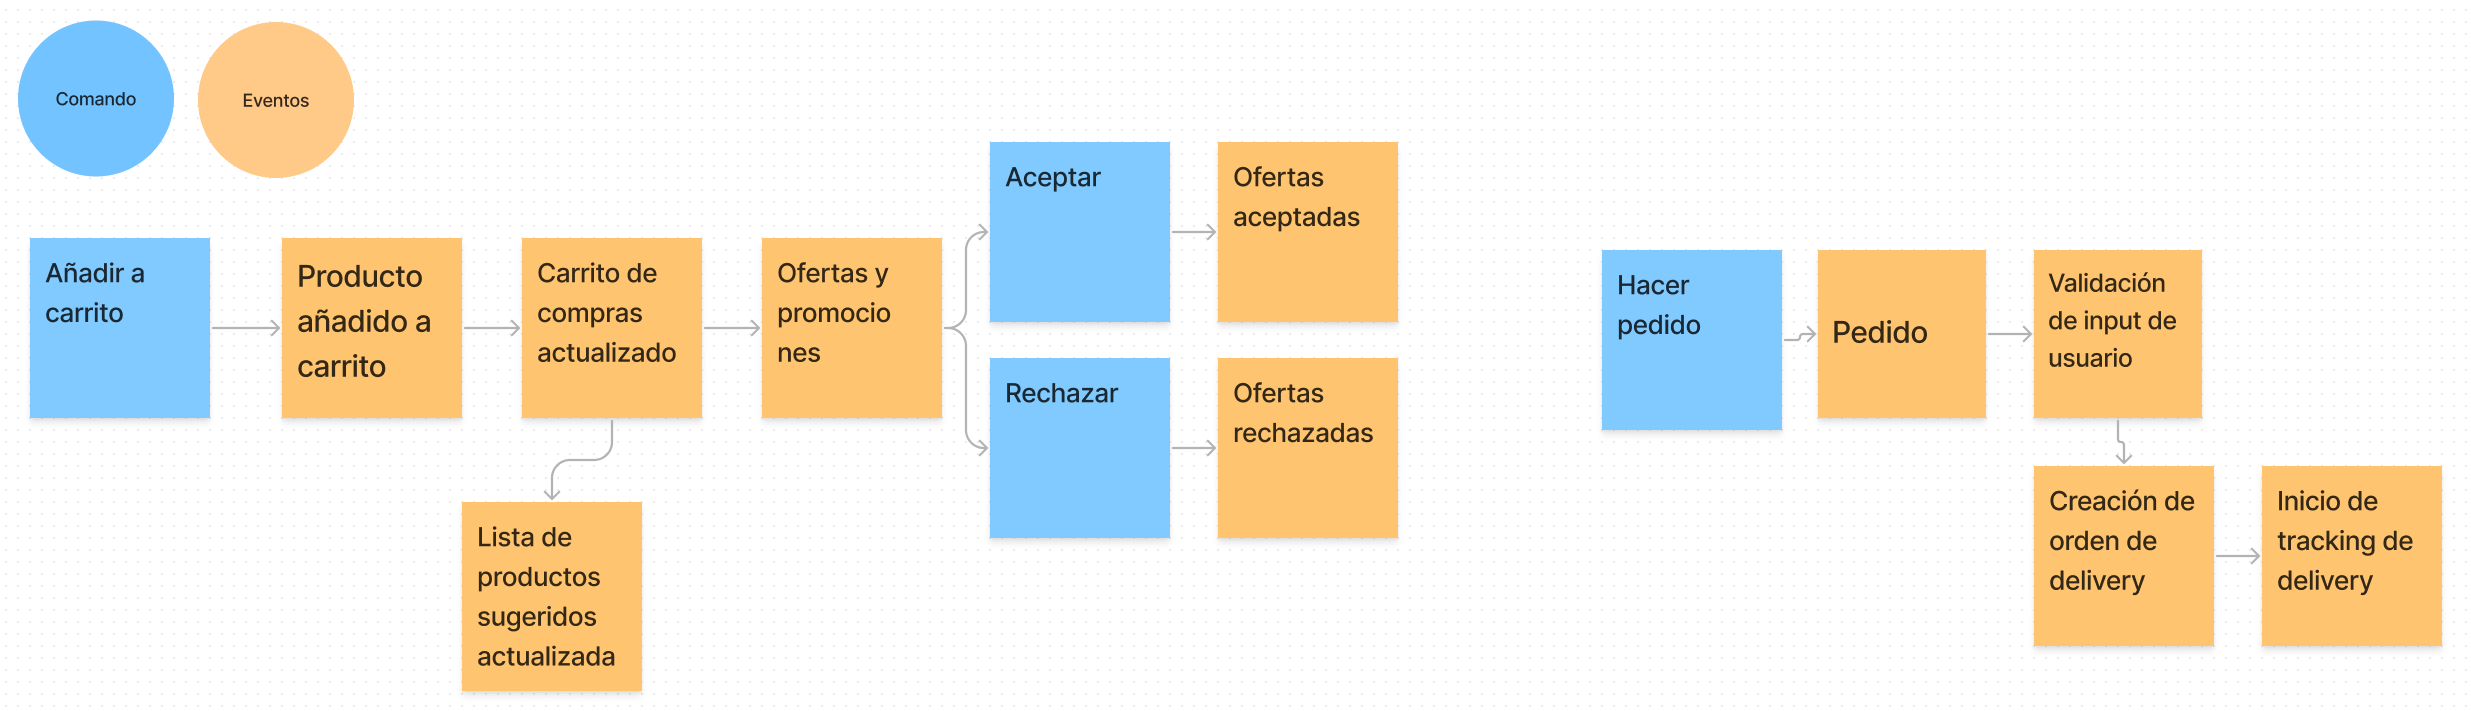
\includegraphics[width=0.90\textwidth]{src/assets/metodologia/event_storming}
    \label{fig:event_storming}
    \end{center}
    Nota: Gráfica de ejemplo de un cuadro producto de una reunión de event storming.
    En este ejemplo se está haciendo la simulación de los eventos de una empresa de e-commerce.
    Elaboración propia.
  \end{figure}

\subsubsection*{Salidas}
\begin{enumerate}[a.]
    \item Identificación de sub-dominios núcleo.
    \item Identificación de sub-dominios de soporte.
    \item Identificación de sub-dominios genéricos.
    \item Modelo de dominio.
    \item Diccionario de términos.
\end{enumerate}


\subsubsection{Definir contextos delimitados}
Luego de identificar los tres tipos de sub-dominios, ya se tiene una visión holística
del sistema que se va a desarrollar pero el modelo de dominio resultante todavía no está
lo suficientemente refinado como para iniciar el desarrollo del sistema.
El dominio todavía tiene relaciones de dependencia, eventos todavía están fuertemente ligados
entre sí, no existe una clara concepción de cómo separar este modelo en microservicios.

De la etapa anterior podemos descartar los sub-dominios genéricos porque pueden ser tercerizados
o en su defecto la organización puede adquirir una solución ya hecha para manejar estos sub-dominios.

Es debido a eso que tomando como base el modelo de dominio se deben definir los contextos delimitados
del modelo.
Para hacer esto hay que apoyarse en las reuniones con los expertos del dominio para identificar
límites entre procesos de la organización.
Una forma para encontrar estos límites lógicos es tomar en cuenta la semántica de las palabras usada por los 
expertos de dominio.

\subsubsection*{Entradas}
\begin{enumerate}[a.]
	\item Sub-dominios núcleo.
	\item Sub-dominios de soporte.
	\item Modelo de dominio.
\end{enumerate}

\subsubsection*{Técnicas y herramientas}
\begin{enumerate}[a.]
	\item Análisis semántico.
  \item Lienzo de contextos delimitados.
\end{enumerate}

\subsubsection*{Ejemplo de la técnica de análisis semántico}

En una entidad financiera el equipo comercial se puede referir a los créditos 
como 'operaciones' mientras que el equipo de cobranzas se refiere a la recaudación de la deuda como 'operaciones'.
Aquí en la misma organización se identifica que la palabra 'operaciones' tiene una semántica diferente entre
estas dos oficinas por lo que hace que se puedan identificar los límites en el modelo de dominio y a su vez 
encontrar los contextos delimitados.


\subsubsection*{Ejemplo de la técnica de lienzo de contextos delimitados}
\vspace{1em}

  \begin{figure}[H]
    % \caption{\\\hspace{\textwidth} Ejemplo de un cuadro de dominio}
    \caption{Ejemplo de un lienzo de contextos delimitados (para un elemento)}
    \begin{center}
    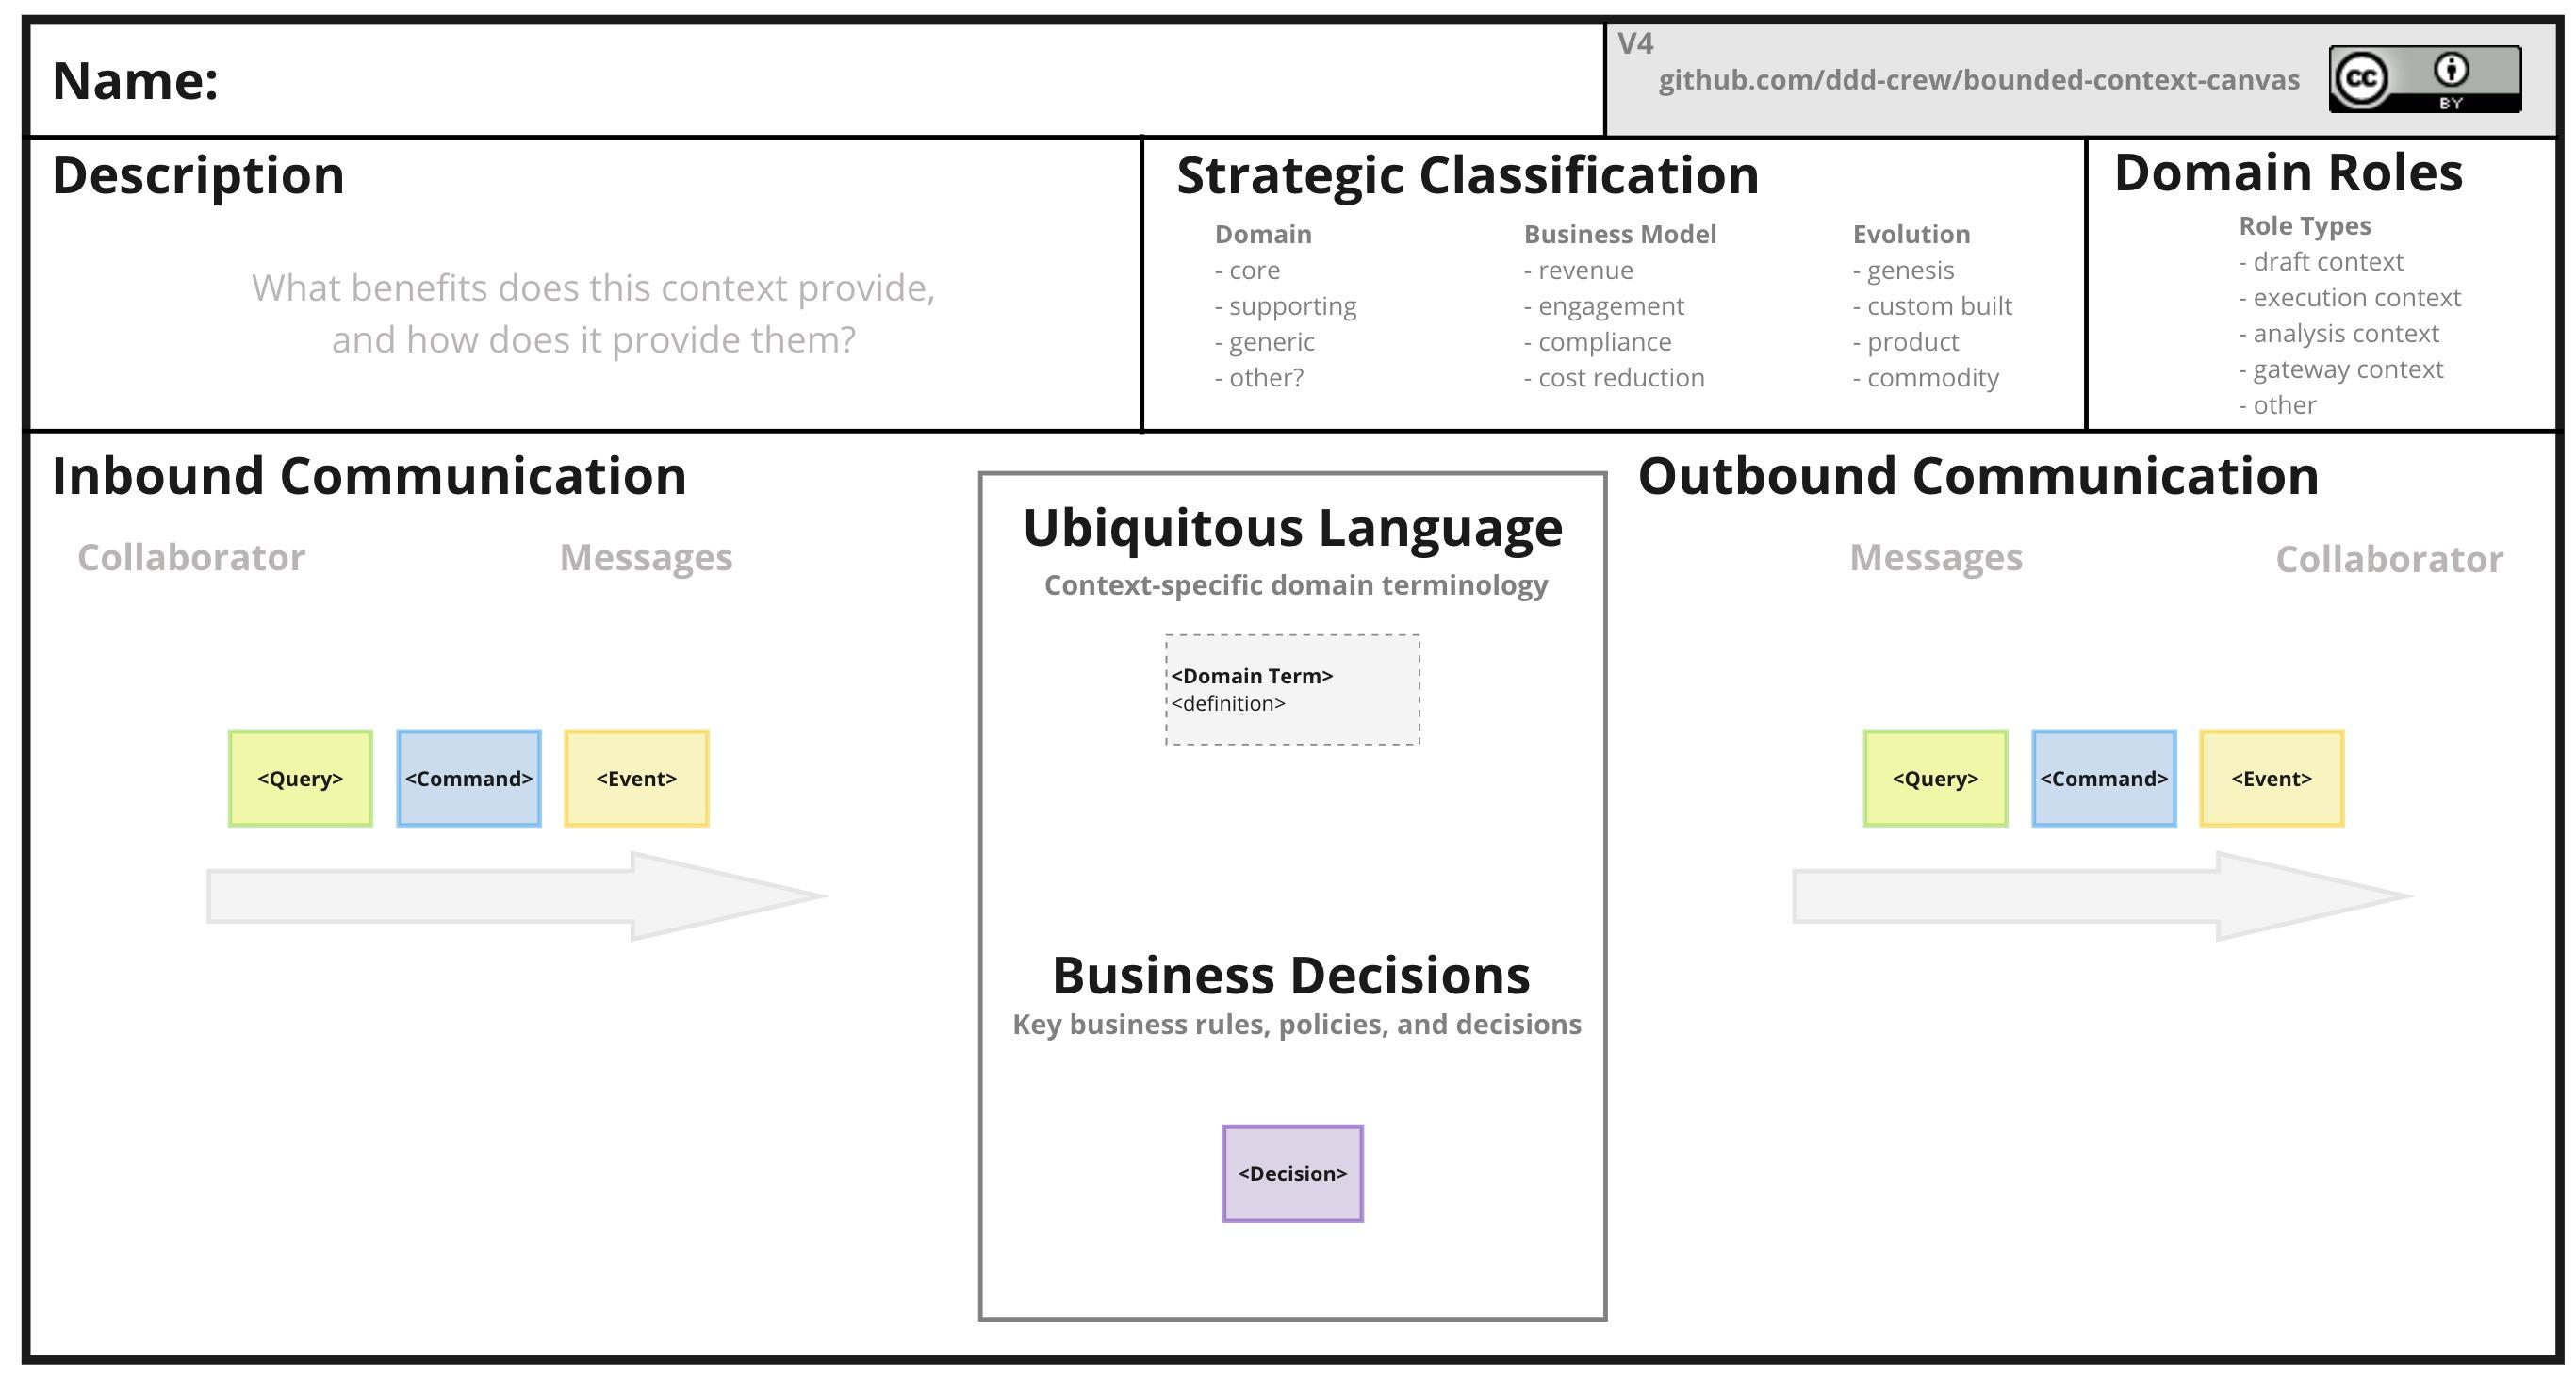
\includegraphics[width=0.90\textwidth]{src/assets/metodologia/bounded_context_canvas}
    \label{fig:bounded_context_canvas}
    \end{center}
    \textit{Nota:} Adaptado de \textit{Bounded Context Canvas}, de \cite{canvas}, Github (shorturl.at/iPVW7). CC-BY-SA-4.0.
  \end{figure}

\subsubsection*{Salidas}
\begin{enumerate}[a.]
    \item Contextos delimitados.
    \item Relaciones de flujos de datos.
\end{enumerate}


\subsubsection{Identificar los microservicios}

Ahora que ya se identificaron los contextos delimitados, ya se pueden identificar los microservicios
juntos formarán nuestra aplicación.
La palabra clave en esta etapa es "identificar", para tener una arquitectura de microservicios que soporte
el despliegue independiente y respete principios de cohesión no se puede forzar definiciones sobre el
dominio de negocio que ya existe, sino que se tienen que identificar y tienen que responder a la realidad.

% TODO https://docs.microsoft.com/es-es/azure/architecture/microservices/model/microservice-boundaries



Entregables propuestos para esta etapa:

\subsection{Crear un ApiGateway como punto de entrada a los servicios}

\subsection{Aseguramiento de la calidad}
